\begin{frame}[fragile]{Proof of Concept: $DP_{WCC}$}
  \begin{itemize}
    \item Develop \underline{\color{red}$WCC$} in \textbf{Haskell} using \acrshort{dp}.
  \end{itemize}
\end{frame}

\begin{frame}[fragile]{Proof of Concept: $DP_{WCC}$}
  \begin{itemize}
    \setlength\itemsep{2em}
    \item {\color{light}Develop $WCC$ in \textbf{Haskell} using \acrshort{dp}.}
    \item Conduct \underline{\color{red}empirical analysis} to prove \textbf{suitability} of implementation
  \end{itemize}
\end{frame}

\begin{frame}[fragile]{Proof of Concept: $DP_{WCC}$}
  \begin{itemize}
    \setlength\itemsep{2em}
    \item {\color{light}Develop the algorithm presented before using \textbf{Haskell}}
    \item {\color{light}Conduct empirical analysis to prove \textbf{suitability} of implementation}
    \item Write an \underline{\color{red}article and present} the results in \textbf{PROLE21 Conference}~\cite{prole:2021:017}
    \item[]
    \item[]
    \item[]
  \end{itemize}
  \begin{textblock*}{7cm}(5cm,4.5cm) % {block width} (coords)
    \fbox{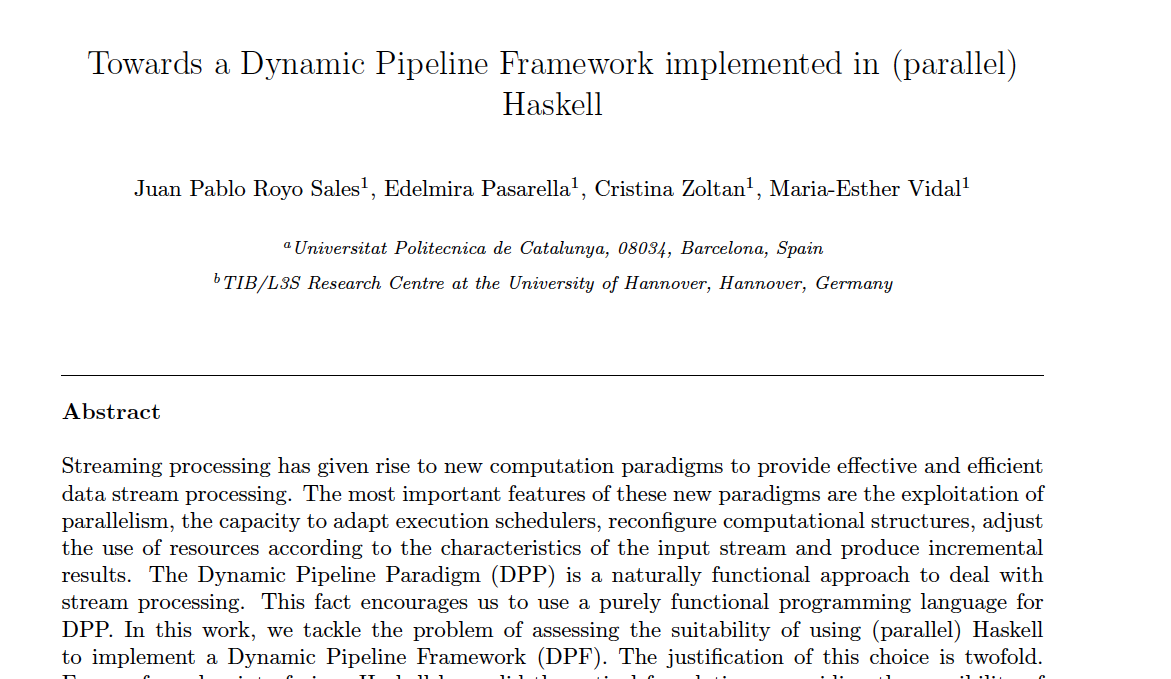
\includegraphics[width = 1\textwidth, height = 0.45\textheight]{paper-prole}}
  \end{textblock*}
\end{frame}

% \begin{frame}[fragile]{Proof of Concept: $DP_{WCC}$ - Empirical Evaluation}
%   \begin{block}{Research Questions}
%     \begin{itemize}
%           \item Does $\dpwcc$ in Haskell support the dynamic parallelization level that $\dpwcc$ requires?
%           \item Is $\dpwcc$ in Haskell competitive compared with default implementations on base libraries for the same problem?
%           \item Does $\dpwcc$ in Haskell handle memory efficiently?
%       \end{itemize}        
%   \end{block}
%   \begin{block}{Experiments}
%     \begin{itemize}
%       \item \textbf{Implementation Analysis}: Measure and analyze Total execution time, MUT time and GC Time.
%       \item \textbf{Benchmark Analysis}: Compare $DP_{WCC}$ with \mintinline{haskell}{Data.Graph} $WCC$ execution times:
%       \begin{itemize}
%         \item Using \mintinline{haskell}{ criterion } library.
%         \item Diefficency metric $\mathtt{dief@t}$ (\textit{diepfy} tool) to measure incremental results.
%       \end{itemize}
%       \item \textbf{Performance Analysis}: Thread and Memory allocation analysis.
%     \end{itemize}
%   \end{block}
% \end{frame}

\begin{frame}[fragile]{Proof of Concept $DP_{WCC}$: Conclusions}
  \begin{itemize}
    \setlength\itemsep{2em}
    \item \underline{\color{red}Robustness and suitability} of the \textbf{DP-Haskell}
    \item Ability to \underline{\color{red}generate incremental results} indicated by higher values of \textbf{$\mathtt{dief@t}$ metric}
    \item \underline{\color{red}Satisfactory performance results} regarding \textbf{Memory allocations and Execution times}. 
  \end{itemize}
\end{frame}

